\documentclass[12 pt, twoside, a4paper] {article}
\usepackage[top=0.8cm, bottom=2cm, left=1cm, right=1cm]{geometry} 
\usepackage[pdftex]{graphicx}
\usepackage{floatrow}
\usepackage{sidecap}
\usepackage{amsmath}
\usepackage{amsfonts}
\usepackage{amssymb}
\usepackage{graphicx}
\usepackage[normalem]{ulem}
\renewcommand{\vec}[1]{\mathbf{#1}}
\let\oldhat\hat
\renewcommand{\hat}[1]{\oldhat{\mathbf{#1}}}
\usepackage{wasysym}     

\begin{document}
\title{Giancoli Ch18:  Kinetic Theory of Gases}
\date{}
\maketitle
\vspace{-50pt}
\textbf{Kinetic theory}: the analysis of matter in terms of atoms in continuous random motion.
$\because$ computational limit $\rightarrow$ can not apply Newton's law to each individual particle$\therefore$ statistical approach (average of quantities= macroscopic variables) 
\vspace{-20pt}
\section{Molecular Interpretation of Temperature}
Postulates of an ideal gas:
\begin{enumerate}
\item large N
\item Separation between molecules $>>$ diameter of molecules
\item Particle interact only classically (i.e. no EM repulsion\/ attraction(?), also quantum mechanics is not considered)
\item Perfectly elastic collision with walls (assume t$\rightarrow$ 0 for collision $\therefore$ in collision $E_p \xrightarrow{completely} E_k$ vice versa (?))
\end{enumerate}
\begin{itemize}
\item Such assumption coincide with Boyle's law;relation between collision probability (surface area ), pressure, and volume (think of a mathematical geometrical proof for this )
\end{itemize}
\subsection{Mechanics applied to gas molecules}
We are trying to find the pressure of gas exert on container:
\begin{align}
\text{Newton's 3rd law}: F_{\text{mcl on wall}} = - F_{\text{wall on mcl}}
						=\frac{dp}{dt} \quad \quad \text{pressure due to collision; assume elastic} \nonumber
\\ \Delta p = 2mV_x  \text{ for each collision each collision separated by time $\Delta$ t}\nonumber
\end{align} 
this is also the time required for one molecules to travel across the container and back again
\\$$\therefore x=2l \rightarrow \Delta t = \frac{2l}{V_x}$$
\\ $$ F= \frac{\Delta p}{\Delta t}= \frac{2 m V_x}{\frac{2l}{V_x}}=\frac{m(V_x)^2}{l}$$
\\ We do not take into account:
\begin{enumerate}
\item V lost by collision with other mcl $\because$ statistically if we $\Sigma$ up, V $\approx$ same
\item Collision with top and bottom $\because$ will not alter $V_x$ component
\item force from collision at intervals $\because$ large N undergo collision $\rightarrow 
F_{avrg} \approx$ constant
\end{enumerate}
\begin{gather*}
F_{\text{due to all molecules}}=\Sigma F_{\text{one molecule}}=\frac{m}{l} (V_{x1}^2+ V_{x2}^2+ \cdots +V_{xN}^2)
\\ \overline{V_x^2}=\frac{(V_{x1}^2+ V_{x2}^2+ \cdots +V_{xN}^2)}{N}
\\ N \overline{V_x^2}=(V_{x1}^2+ V_{x2}^2+ \cdots +V_{xN}^2)
\\  F=\frac{m}{l}N\overline{V^2_x} \because \text{velocity random, we assume}\overline{V_x}= \overline{V_y}=\overline{V_z} 
\\ \because \overline{V}=\overline{V_x}^2+\overline{V_y}^2+\overline{V_z}^2=3\overline{V_x}
\\ F=\frac{m}{l}N\frac{\overline{V_x}}{3}
\\ P=\frac{F}{A}=\frac{\frac{m}{l}N\frac{\overline{V}}{3}}{A} 
\\ \because \textbf{V}=\text{volume}=Al \quad\quad\quad\quad\quad P\textbf{V}= \frac{2}{3} N(\frac{1}{2} m \overline{V}^2) \quad\quad\text{ and }\quad\quad P\textbf{V}=NkT
\\kT= \frac{2}{3} (\frac{1}{2} m \overline{V}^2)= \frac{2}{3} \tau \quad \quad \text{  where $\tau$ is kinetic energy}
\end{gather*}
\begin{equation}
\therefore  \tau=\frac{3}{2}kT
\end{equation}
This is also a reasonably accurate prediction for how fast molecules move on average in liquids and solids.
$$\tau=\frac{1}{2} m \overline{V}^2 =\frac{3}{2}kT$$
\begin{equation}
\therefore \text{Root mean square velocity}= V_{rms}=\sqrt{\overline{V}^2}=\sqrt{\frac{3kT}{m}}
\end{equation}
Kinetic Energy near absolute zero:
The $V_{rms}$ formula implies that as $T \rightarrow 0$ then $V_{rms} \rightarrow 0$
\\Quantum Mech: as $T \rightarrow 0$ then $V_{rms} \rightarrow $small nonzero minimum value.Even at abs zero, molecular motion doesn't cease (even though macroscopically the substance has  probably transformed into a solid or liquid)
\section{Distribution of Molecular Speeds}
\subsection{Maxwell Distribution}
Probable distribution of speeds in a gas containing N molecules
\begin{equation}
f(v)= 4\pi N (\frac{m}{2 \pi k T})^{\frac{3}{2}} v^2 e^{-\frac{1}{2}\frac{mv^2}{kT}}
\end{equation}
\begin{itemize}
\item v:Relative number of molecules
\item m: mass of a single molecule
\end{itemize}
\subsection{Temperature dependent}
\begin{itemize}
\item not symmetrical distribution skewed to the right
\item Temperature $\uparrow$ then distribution shift to the right
\item $\because$ this way larger portion exceeds $E_a$ threshold
\end{itemize}
\subsection{Calculations}
\begin{itemize}
\item Finding $\overline{v}: $
\\$ f(v) dv\rightarrow $number of mcl that have speed between v and v+dv
\\ Taking lim dv$\rightarrow$0, we see that $ f(v) dv$ = number of molecules that has a specific speed$_i$
\footnote{ $\therefore$ total number of molecules in gas(N)=$\int^\infty_0 f(v)$}
$$\overline{v}=\frac{\Sigma \text{probability of speed$_i$}\times \text{number of molecules that has speed$_i$}} {N}$$
Again taking the limit for integration, we get a formula for average speed
$$\overline{v}=\frac{\int_0^\infty v f(v) dv } {N}$$
Through tedious integration (which I haven't attempted),
$$\overline{v}=\sqrt{\frac{8}{\pi}\frac{kT}{m}}\approx1.60 \sqrt{\frac{kT}{m}}$$
\item Finding most probable speed ($V_p$):
\\By observing the Maxwell distribution (which resembles a Gaussian curve), intuitively the most probable speed is at the maximum. Simple optimization $\frac{df(v)}{dt}=0$ yields our value for $V_p$\footnote{There are two solutions, find the one that yields the maxiumum}
$$V_p=\sqrt{\frac{2kT}{m}}\approx 1.41\sqrt{\frac{kT}{m}} \quad \quad \quad \quad
\footnote{Recall $V_{rms}=\sqrt{\frac{3kT}{m}}\approx 1.73\sqrt{\frac{kT}{m}}$, we again confirm that all speeds are smaller than $V_{rms}$}$$
\end{itemize}
\section{Real Gases and Change of Phase}
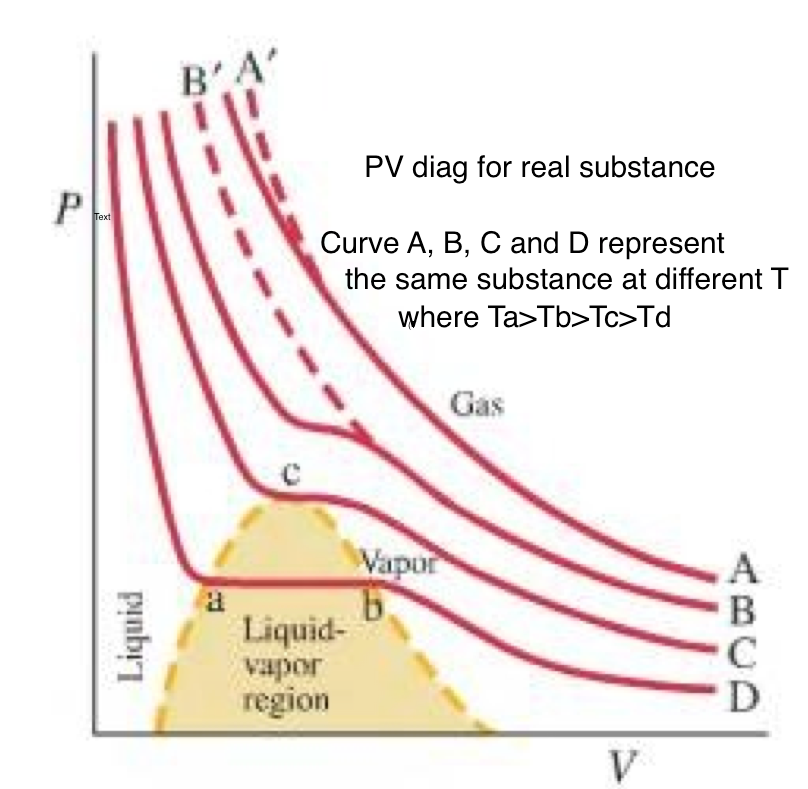
\includegraphics[scale=0.2]{RealGasPVDiagram2}
\begin{itemize}
\item The dotted line is the ideal gas prediction. At lower temperature (A) real gas $\rightarrow$ ideal
\item Our ideal gas postulate 4 breaks down, $\because E_p $\footnote{1)lower temperature ($\approx$ liquefaction) higher pressure , molecules closer, $\therefore E_p $of attractive force $\uparrow$ \\2) as temperature lowers (s.t. T $\rightarrow$ b.p.), $E_k \downarrow$, so $E_k$ no longer $>> E_p \therefore$ must take $E_p$ into consideration \\3) V-nb volume consideration (gas compressible $\rightarrow$liquid $\approx$ incompressible)} no longer negligible
\item Critical temperature($T_c$) occur @ critical point
\item Critical point is where curve on graph is horizontal
\item If T $< T_c$, (g)$\rightarrow$ (l) if you apply sufficient pressure
\item But if T$> T_c$, even $\infty$ pressure can not cause (g)$\rightarrow$ (l)
\item \textbf{Vapor}: substance in a gaseous state when  T $< T_c$ (artificially made so it's like that)
\item \textbf{Gas}: substance in a gaseous state when T  $>T_c$ (naturally like that)
\end{itemize}
\subsection{PT diagram (a.k.a Phase diagram)}
\begin{figure}[h!]
\center
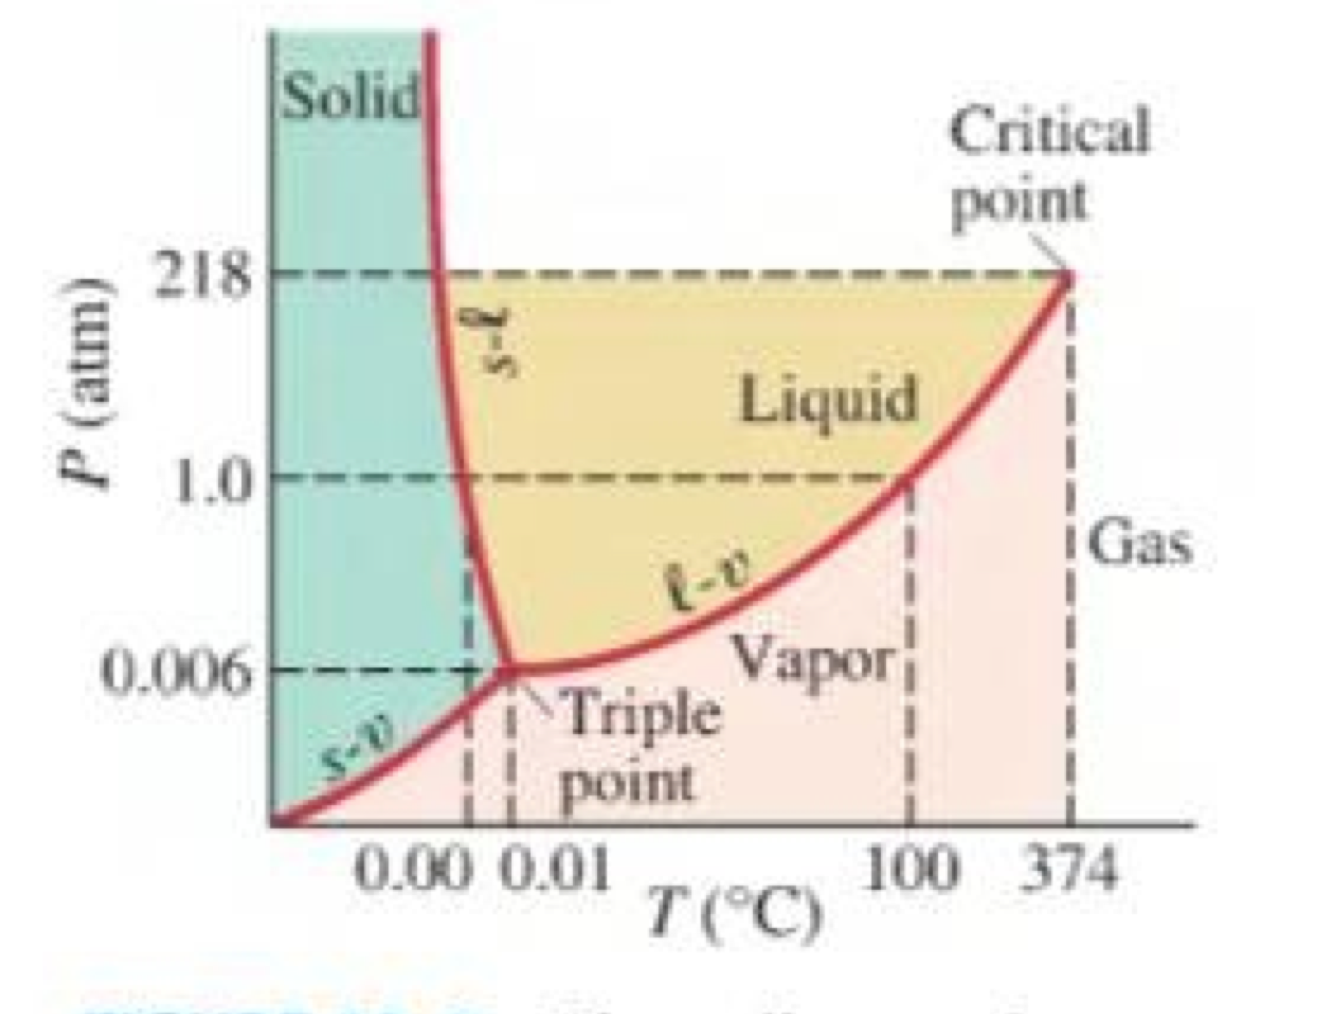
\includegraphics[scale=0.3]{PhaseDiagramWater}
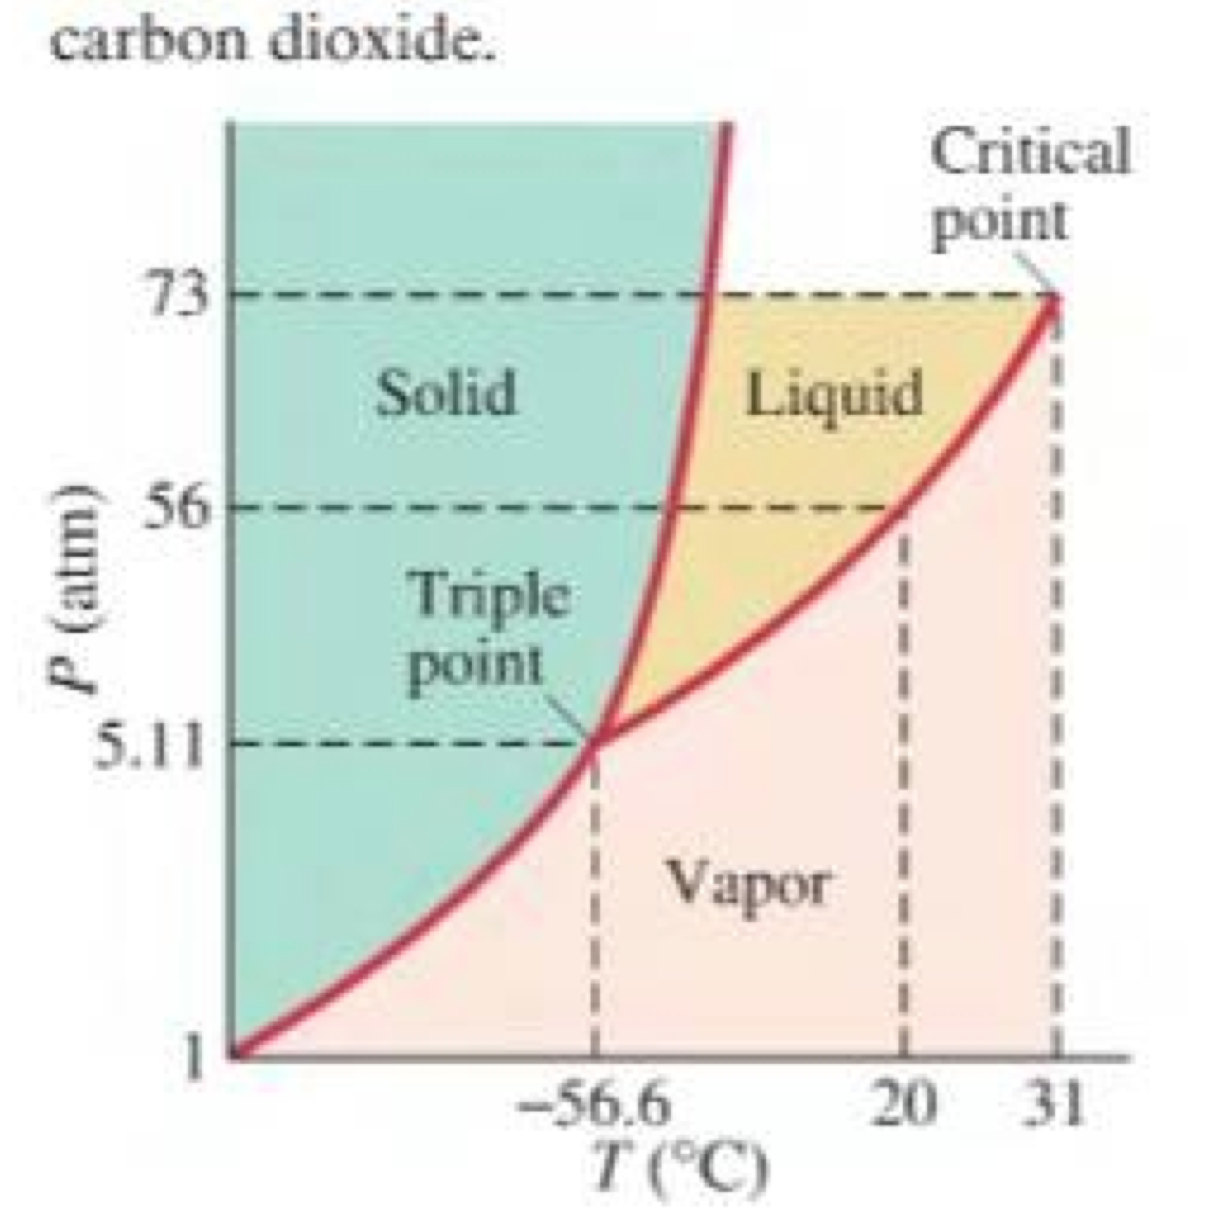
\includegraphics[scale=0.3]{PhaseDiagramCO2} 
\vspace{-10pt}
\caption{Right: Water; Left: CO2}
\end{figure}
\begin{itemize}
\item Curve: values of P and T for which the two indicated phases coexist in equilibrium
\item Triple Point:three phases coexist in equilibrium\footnote{Sublimation : @ low pressure, (s) $\rightarrow$(g)}
\item s-l curve: slope up-leftward if substance expands while freezing  $\because$ given a higher pressure , it will require lower pressure to freeze \footnote{Think of this as stuff being further apart so they are harder to freeze}
\item Most substance contract while freezing $\therefore$ slope right-leftward \footnote{The same reasoning applies, given a higher pressure, it will require less lower pressure to freeze since it contracted relative to the initial point where it began freezing (at that initial point: normal-sized)}
\item Phase transition can also occur in the same phase. (e.g. Helium has two forms in liquid phase, Helium II :superfluid ( 0 viscocity, wall climbing)
\item LCD (liquid crystal) are in a phase between solid and liquid  (Is this talking about plasma??)
\end{itemize}

\section{Vapor Pressure and Humidity}
\subsection{$P_{vap}$ and Evaporation}
\begin{itemize}
\item Evaporation occurs when high-speed surface atoms \footnote{Speed of particles $\approx$ follow Maxwell distribution} in a liquid escape into air
\item Evaporation is a cooling process $\because$ high T$\rightarrow$ high V, all high V escape, $\therefore$ average V is lower$\rightarrow$average temperature lower
\item Equal rates of condensation and evaporation $\rightarrow$ equilibrium
\item If $\leftrightarrow$ then space above liquid surface: \textbf{saturated}
\item \textbf{(Saturated) vapor pressure}:pressure of vapor when it is saturated 
\item Vapor pressure independent of volume $\because$ if V $\downarrow$ then $\rho_{molecule} \uparrow$. $\frac{\mathrm d}{\mathrm dt} \mathrm (Condensation)>>\frac{\mathrm d}{\mathrm dt} \mathrm (Evaporation)$ so that vapor pressure is maintained
\item Vapor pressure depend on Temp $\because$ high T $\rightarrow$ large $E_k \rightarrow$ surface mcl escape $\rightarrow P_{vap} \uparrow$ then reach equilibrium (@ the new higher $P_{vap}$)
\end{itemize}
\subsection{Boiling}
\begin{itemize}
\item $P_{vap} \uparrow$ as T $\uparrow$ until $P_{vap} = P_{external} \rightarrow$ boiling
\item Bubble at surface: Initially collapse $\because P_{inside} < P_{external}$
\item Once $P_{inside} \geq P_{external}$, bubble rise up : (l) $\rightarrow$ (g) $\therefore$ boiling occurs \footnote{1atm = 760 torr}
\item Ex) Pressure cooking v.s. high-altitude cooking
\end{itemize}
\subsection{Partial Pressure and Humidity}
\footnote{Supersaturate: $P_{H_2O \quad partial }>P_{vap}$}
\footnote{\textbf{Dew point}: temperature at which $P_{H_2O \quad partial }=P_{vap}$}
Partial pressure: the pressure each gas would exert if it alone were present (0$\leq P_{partial} \leq P_{vap}$)
\\Total pressure of gas mixture= $\Sigma$ partial pressure of each gas
$$\text {Relative humidity at a given temperature}= \frac{\text{partial pressure of $H_2O$}}{\text{saturated vapor pressure of $H_2O$}} \times100\%$$
\section{Van der Waals Equation of State}
\subsection{Van der Waals gas}
Ideal gas but take into account:\begin{enumerate}
\item molecule has finite non-zero size compared to $V_{container}$
unavailable volume is what the molecule takes up, it is dependent of the size and number of the molecules.(nb)
\begin{equation}
\therefore V_{\text{actual}}=V-nb
\end{equation}
Using this in ideal gas law and dividing by n, we get \textbf{Clausis equation of state}:
\begin{equation}
P(\frac{V}{n}-b)=RT
\end{equation}
This tells us that $P_{real}> P_{ideal}$, which makes intuitive sense because as V $\downarrow \rightarrow$ more collision$\rightarrow P \uparrow$
\item the intermoecular force may be greater than size if moecule assume to be hard spheres colliding
\begin{itemize}
\item Intermolecular force is:
\begin{itemize}
\item small range
\item hodl molecules in (l) and (s) @ low T
\item Electrical in nature
\end{itemize}
\item Inward attractive force oppose the pressure on walls
\item the magnitude of this force decrease with each shell (?)

\item proportional to shell density in each shell layer $\alpha (\frac{n}{V})^2 $
\item $$P_{actual}= P+\frac{a}{(\frac{V}{n})^2 }$$
\item Fig 18-11 (?)
\end{itemize}
\end{enumerate}
\subsection{Equation of state}
\begin{itemize}
\item $$\therefore (P+\frac{a}{(\frac{V}{n})^2})(\frac{V}{n}-b)=RT$$
\begin{equation}
\text{Van der Waals equation of state}\quad \quad P=\frac{RT}{(\frac{V}{n}-b)}-\frac{a}{(\frac{V}{n})^2} 
\end{equation}
\item This is a closer approximation of real gas but only with the improvement of removal of 2 assumption. No proposed equation of state is accurate for all gas under all condition. 
\item Van der Waal happens to be useful under many conditions. 
\item @ low $\rho$ : $\frac{a}{(\frac{V}{n})^2}<<P$ and $\frac{V}{n}>>b$ so the equation reduces back to ideal gas law PV=nRT
\end{itemize}
\section{Mean Free Path}
\begin{itemize}
\item particular molecule follow zigzag path $\because$ multiple collision with other molecules
\item \textbf{Mean-free path}: average distance travelled between each collision.
\item Assumptions:
\vspace{-10pt}
\begin{enumerate}
\item ignore intermolecular force
\item ideal gas
\item assume other particles are stationary\footnote{Our use of $V_{relative}$later in the derivation accoutns for this}
\end{enumerate}
\item \begin{figure}[h]
\vspace{-10pt}
\floatbox[{\capbeside\thisfloatsetup{capbesideposition={left,top},capbesidewidth=7cm}}]{figure}[\FBwidth]
{\caption{
height of cylinder=v$\Delta$t  \newline
volume of cylinder=$\pi (2r)^2(v\Delta t)$  \newline
$ \text{\# of collision per sec} =\frac{N}{V_{molecule}}V_{cylinder}=\frac{N}{V_{molecule}}\pi (2r)^2(v\Delta t)$
}\label{fig:test}}
{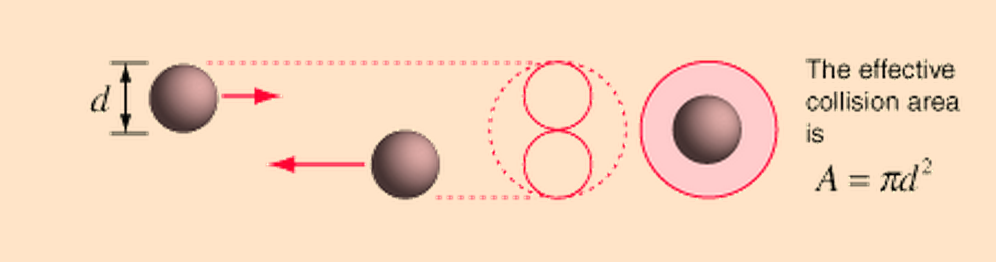
\includegraphics[width=9cm, scale=0.5]{EffectiveArea}}
\end{figure}
\vspace{-10pt}
%\begin{SCfigure}[h]
%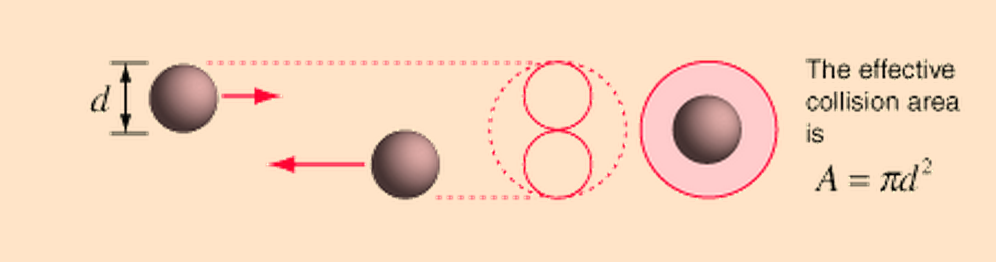
\includegraphics[scale=0.5]{EffectiveArea}
%$A_e$ =effective area of collision= $\pi (2r)^2$
%\caption{height of cylinder=v$\Delta$t  \newline
%volume of cylinder=$\pi (2r)^2(v\Delta t)$  \newline
%number of collision per second=$\frac{N}{V_{molecule}}V_{cylinder}
%\newline \quad \quad \quad \quad =\frac{N}{V_{molecule}}\pi (2r)^2(v\Delta t)$}
%\end{SCfigure}
$$l_m=\frac{\text{distance travelled in time $\Delta$ t}}{\text{number of collision in time $\Delta$ t}}=\frac{\overline{v}\Delta t}{\frac{N}{V}\pi(2r)^2 (v_{relative}\Delta t)}$$
From Maxwell's distribution, we find that: $$v_{relative}=\sqrt{2}\overline{v}$$
\begin{equation}
\therefore l_m=\frac{1}{4r^2\sqrt{2}\pi\frac{N}{V}}
\end{equation} 
\item $l_m$ looses meaning at low $\rho \because$ collision frequency with wall$> $collision frequency with other molecules (ex. when $l_m>$length of box)
\end{itemize}

\section{Diffusion}
\begin{itemize}
\item C : concentration
\item J : rate of diffusion=$\frac{\# of molecules diffusing across the area}{\Delta t}=\frac{N}{\Delta t}$
\item J $\alpha \text{concentration gradient}=\frac{\Delta C}{\Delta x}$
\item Fick's Law(Diffusion equation)\footnote{make sure the units for J, C correspond to each other } :
	\begin{equation}
		J= DA \frac{\Delta C}{\Delta x}= DA\frac{dC}{dx}
	\end{equation}		
\item can use definitions, and various trivial things to solve for t: $t\approx\frac{\Delta x ^2}{D}$
\end{itemize}
\section{Question}
\begin{itemize}
\item pg 477 ``molecules exert weak attractive force on each other between collisions", if molecules are of the same charge ,which they should be? Shouldn't the force be repulsive?
\item How does this work? t$\rightarrow$ 0 for collision $\therefore$ in collision $E_p \xrightarrow{completely} E_k$
\item LCD (liquid crystal) are in a phase between solid and liquid  (Is this talking about plasma??)
\item During pg 477 derivation, why do we need to consider back and forth across container (2l) instead of simply using l?
\item pg486 Excercise E : Why is answer b)decrease?
\item for Van der Waals equation why is proportional to shell density in each shell layer $\alpha (\frac{n}{V})^2 $?  (surface area of shell?volume of shell?)
\end{itemize}

$\quad \quad \quad  \quad \quad \quad \quad \quad \quad \quad \quad \quad \quad \quad \quad \quad \quad \quad \quad \quad \quad \quad \quad \quad \quad \quad \quad \quad \quad \quad \quad \textbf{Last Update:\today}$
\end{document}